\section{Weigthed Shortest Job First}
	
	Para a priorização das features identificadas, foi utilizado o conceito do SAFe da tabela WSJF (Weighted Shortest Job First), que leva em consideração quatro fatores para a sua priorização, são eles: \textbf{Busines Value, Time Criticality, Risk Reduction} e \textbf{Job Size}.  Ela tem como objetivo priorizar as features que agregam maior valor ao negócio e que são mais rápidas de serem implementadas. A feature que possuir o maior valor WSJF deverá ser implementada primeiro. (Scaled Agile Framework, 2015).

	O \textbf{Busines Value} diz respeito ao valor de negócio que a feature representa para o sistema no geral. Para calcular, deve ser levado em consideração se essa feature traz impactos ao negócio, ou seja, se ela é de maior importância para o negócio que as outras. (Scaled Agile Framework, 2015).

	O \textbf{Time Criticality} diz respeito à importância de uma feature ser desenvolvida em um curto prazo de tempo. Tem que ser levado em consideração se essa feature só agrega valor ao negócio se for produzida até um prazo estabelecido e quanto o valor de negócio dessa feature decai de acordo com o prazo de desenvolvimento. (Scaled Agile Framework, 2015).

	O \textbf{Risk Reduction-Opportunity Enablement Value} diz respeito ao quanto que essa feature pode reduzir o risco de uma outra funcionalidade, gerando resultados que serão consumidos posteriormente e proporcionando novas oportunidades ao negócio. (Scaled Agile Framework, 2015).

	O \textbf{Job Size} é o tamanho da feature. Nesse ponto, a que demanda mais tempo para ser implementada possui um Job Size maior. (Scaled Agile Framework, 2015).

	Para a construção da WSJF, houve uma uma reunião com o cliente em que foi-se conduzida uma conversa que possibilitou a identificação de valores a serem atribuídos para cada um dos fatores de priorização utilizados na tabela. Para a obtenção desses fatores, realizou-se primeiramente a identificação do item de menor valor e, a partir dele, obtiveram-se os valores correspondentes das próximas features. Após o preenchimento da tabela, foi utilizada a fórmula fornecida que pode ser verificada abaixo, para calcular a coluna WSJF.

	\newpage
	\vspace*{5mm}
	\begin{table}[htbp]
		\centering
		\begin{tabular}{c c}
			& \textbf{User|Business Value + Time Criticality + RR|OE Value} \\
			\textbf{WSJF} = & ---------------------------------------------------- \\
			 & \textbf{Job Size}
		\end{tabular}
	\end{table}

	\vspace*{2cm}

	\noindent
	\textbf{BV} = Business Value;\\
	\textbf{TC} = Time Criticality.\\


	\begin{table}[!htp]
		\caption{Tabela WSJF}
		\begin{tabular}{|l|l|l|l|l|l|l|}
			\hline
			\textbf{Tag} & \textbf{Feature} & \textbf{BV} & \textbf{TC} & \textbf{RR/OE} & \textbf{Job Size} & \textbf{WSJF} \\ \hline

			FEAT-3.8 & Manutenção de Usuários & 13 & 8 & 20 & 3 & 13.7\\ \hline

			FEAT-1.2 & Manutenção de PRP & 3 & 2 & 20 & 3 & 8.3 \\ \hline

			FEAT-1.1 & Manutenção da DRP & 3 & 1 & 13 & 3 & 5.7 \\ \hline

			FEAT-1.3 & Validação de PRP & 1 & 2 & 20 & 5 & 4.6 \\ \hline

			FEAT-1.4 & Manutenção da QP & 5 & 2 & 13 & 5 & 4.0 \\ \hline

			FEAT-2.5 & Resposta QP & 8 & 5 & 5 & 5 & 3.6 \\ \hline

			FEAT-2.7 & Geração de Relatório Estatístico & 8 & 5 & 1 & 8 & 1.7 \\ \hline

			FEAT-2.6 & Geração de Relatório Semântico & 8 & 5 & 1 & 20 & 0.7 \\ \hline
		\end{tabular}
	\label{Tabela WSJF}
	\end{table}

	\begin{landscape}
	\begin{figure}[h]
		\vspace*{11mm}
		\centering
		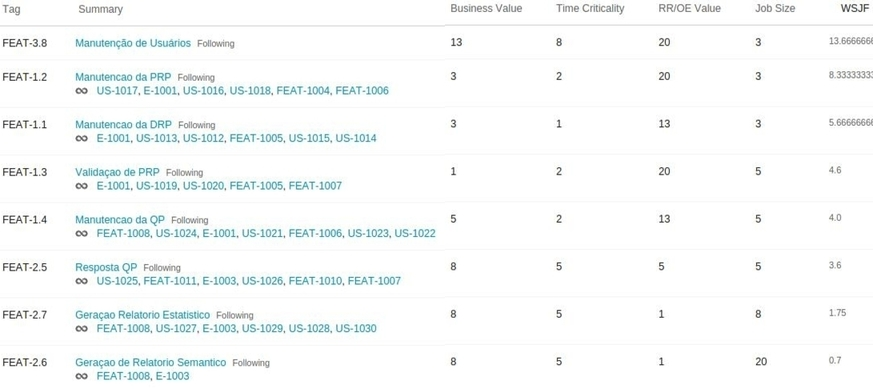
\includegraphics{imagens/wsjf3.jpg}
		\caption{Tabela wsjf na ferramenta.}
		\label{imagem}
	\end{figure}
	\end{landscape}


